\chapter{Desenvolvimento do controlador}
\label{ch:desenvolvimento_controlador}

Com o intuito de controlar o \acrshort{tclabsp} aplicando o \acrshort{mpc} como técnica,
utilizaram-se os modelos teóricos e experimentais apresentados na \cref{sec:modelagem_da_planta_piloto}
e na \cref{sec:modelo_experimental} para o desenvolvimento do bloco controlador no \textit{Simulink}.
Um controlador \acrshort{pid} também foi desenvolvido a fim de servir como base comparativa ao
controlador \acrshort{mpc} criado.
A seção a seguir descreve este controlador \acrshort{pid}.

% =====================================================================================================
% ============================================= Section ===============================================
% =====================================================================================================
\section{Controlador PID}
\label{sec:controlador_pid}

O controlador \acrshort{pid} desenvolvido foi criado em ambiente \textit{Simulink},
utilizando o aplicativo \textit{PID Tuner} do \acrshort{matlab}, disponível através do pacote
\textit{Control System Toolbox}.

A cada um dos Aquecedores do \acrshort{tclabsp} foi conectado a um bloco \textit{PID Controller} retroalimentado
com a saída dos Sensores de Temperatura da planta, conforme ilustrado pela \cref{fig:pidcreation}.

\begin{figure}[h]
	\caption{Modelo Simulink do controlador PID}
	\begin{center}
		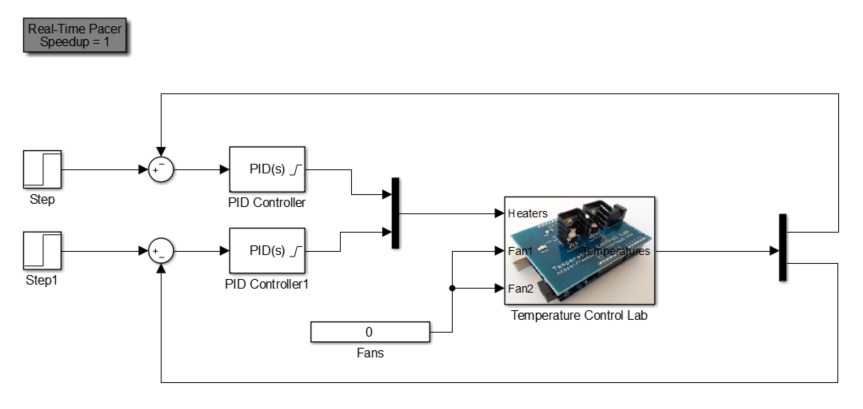
\includegraphics[width=1.00\textwidth]{./5_images/PIDCreation.png} 
		\label{fig:pidcreation}
	\end{center}
	\centering
	\makebox[\width]{Fonte: Autor} 
\end{figure}

Os blocos \textit{PID Controller} foram inicialmente configurados com os limites de saturação de saída
entre 0 e 100 para que nenhum valor fora desta faixa fosse aplicado a planta controlada.
Em seguida, uma vez que o desenvolvimento do controlador \acrshort{pid} não era um objetivo deste trabalho,
utilizou-se a função de auto-sintonia do \textit{PID Tuner} para encontrar valores satisfatórios de controle
do sistema.

A \cref{tab:pid_values} apresenta os valores de sintonia encontrados para um controlador \acrshort{pid}
paralelo (\cref{eq:pid_format}).

\begin{equation}
    \label{eq:pid_format}
    P + I \frac{1}{s} + D \frac{N}{1 + N \frac{1}{s}}
\end{equation}

\begin{table}[h]
	\centering
	\caption{Sintonia dos blocos PID}
	\label{tab:pid_values}
	\begin{tabular}{c|cc} \toprule
		{Parâmetro}		            & {PID Aquecedor 1}     & {PID Aquecedor 2}           \\ \midrule
		Proporcional (P)		    & $1.435$               & $2.182$                     \\
		Integral (I)   		        & $0.016$               & $0.011$                     \\
		Derivativo (D)		        & $-9.119$              & $-30.919$                   \\
		Filtro (N)                  & $0.0216$              & $0.010$                     \\ \bottomrule
	\end{tabular}
	\caption*{Fonte: Autor}
\end{table}


% =====================================================================================================
% ============================================= Section ===============================================
% =====================================================================================================
\section{Controlador MPC}
\label{sec:controlador_mpc}

Segundo \citeonline{Alhajeri2020}, o grande número de parâmetros sintonizáveis motivou diversos estudos
sobre como sintonizar o \acrshort{mpc} e nesta seção serão indicadas as técnicas utilizadas na sintonia de cada
um dos parâmetros do controle \acrshort{mpc} em questão.

% .....................................................................................................
% ............................................ Subsection .............................................
% .....................................................................................................
\subsection{Horizonte de predição}
\label{subsec:horizonte_de_predicao}

A janela de tempo que especifica quantos períodos de amostragem futuros sobre os quais a resposta da 
variável controlada $y_i$ será predita pelo modelo da planta e então otimizada é chamado de horizonte
de predição \cite{Alhajeri2020}. Este horizonte é indicado pela letra $P$ e seus limites inferiores
e superiores são, respectivamente, $P_{0_{n_y}}$ e $P_{n_y}$. Importante notar que o horizonte de predição
é calculado para cada saída $n_y$, portanto em um sistema com 2 saídas, por exemplo, os limites inferiores
serão $P_{0_1}$ e $P_{0_2}$ e os limites superiores $P_1$ e $P_2$.

No seu estudo sobre as diferentes técnicas de sintonia do \acrshort{mpc}, \citeonline{Alhajeri2020} indicam
que, no geral, o horizonte de predição deve ser adequadamente grande para que as predições das saídas
controladas possam representar uma porção significativa do processo, portanto valores altos devem
ser selecionados para $P_1$, $\cdots$, $P_{n_y}$, para assegurar a estabilidade e robustez em malha fechada.
Contudo, quanto maiores forem estes valores, maior será o custo computacional para a resolução do
problema de otimização do \acrshort{mpc}. Na prática, aumentar os valores de $P_1$, $\cdots$, $P_{n_y}$
aumenta a robustez e a estabilidade, porém após certos valores o aumento desta janela de predição não
altera a performance de controle significativamente, mas irá intensificar a carga computacional, o que
pode deteriorar a robustez do controle.

As \cref{eq:horizonte_de_predicao_lim_inf_no_delay,eq:horizonte_de_predicao_lim_inf_with_delay},
sugeridas por \citeonline{Alhajeri2020}, indicam os valores de limite inferior do horizonte de predição
 para plantas sem atraso e com atraso, respectivamente.

\begin{equation}
	\label{eq:horizonte_de_predicao_lim_inf_no_delay}
    P_{0_1} = 1, \cdots, P_{0_{n_y}} = 1
\end{equation}

\begin{equation}
	\label{eq:horizonte_de_predicao_lim_inf_with_delay}
	P_{0_1} = 1 + \frac{\min_j \left( \sum_{j=1}^{n_u} \theta_{1_j} \right)}{t_s}		\\
	, \cdots,																			\\
	P_{0_{n_y}} = 1 + \frac{\min_j \left( \sum_{j=1}^{n_u} \theta_{{n_y}_j} \right)}{t_s}
\end{equation}

\noindent
Onde: 
\begin{itemize}
	\item $n_u$: são as entradas do sistema
	\item $\theta_i$: é o tempo morto da planta
	\item $t_s$: é o período de amostragem
\end{itemize}

Os mesmos autores indicam estudos que sugerem que o limite superior seja calculados segundo
as \cref{eq:horizonte_de_predicao_lim_sup_no_delay,eq:horizonte_de_predicao_lim_sup_with_delay},
sendo a primeira sem a utilização de tempo morto, e a segunda, considerando o tempo morto da planta.

\begin{equation}
	\label{eq:horizonte_de_predicao_lim_sup_no_delay}
    P_{1} = \frac{0.8 * T_s}{t_s} , \cdots, P_{{n_y}} = \frac{0.8 * T_s}{t_s}
\end{equation}

\begin{equation}
	\label{eq:horizonte_de_predicao_lim_sup_with_delay}
	\begin{aligned}
		\frac{\max_j \left( \sum_{j=1}^{n_u} \theta_{1_j} \right)}{t_s} + 1					
		\leqslant P_1 \leqslant																
		\frac{\max_j \left( \sum_{j=1}^{n_u} \theta_{1_j} \right)}{t_s} + 					
		\max_J \left( \sum_{j=1}^{n_u} M_j \right)											
		, \cdots,																			\\
		\frac{\max_j \left( \sum_{j=1}^{n_u} \theta_{{n_y}_j} \right)}{t_s} + 1				
		\leqslant P_{n_y} \leqslant															
		\frac{\max_j \left( \sum_{j=1}^{n_u} \theta_{{n_y}_j} \right)}{t_s} + 				
		\max_J \left( \sum_{j=1}^{n_u} M_j \right)
	\end{aligned}
\end{equation}

\noindent
Onde: 
\begin{itemize}
	\item $n_u$: são as entradas do sistema
	\item $\theta_i$: é o tempo morto da planta
	\item $t_s$: é o período de amostragem
	\item $T_s$: é o maior tempo de acomodação das variáveis controladas em malha aberta
	\item $M_i$: é o horizonte de controle 
\end{itemize}

% .....................................................................................................
% ............................................ Subsection .............................................
% .....................................................................................................
\subsection{Horizonte de controle}
\label{subsec:horizonte_de_controle}

